% \documentclass[12pt, twoside]{article}
\usepackage[letterpaper, margin=1in, headsep=0.2in]{geometry}
\setlength{\headheight}{0.6in}
%\usepackage[english]{babel}
\usepackage[utf8]{inputenc}
\usepackage{microtype}
\usepackage{amsmath}
\usepackage{amssymb}
%\usepackage{amsfonts}
\usepackage[nomessages]{fp} %\FPeval{\var-name}{2*sin(pi/6)}
\usepackage{siunitx} %units in math. eg 20\milli\meter
\usepackage{yhmath} % for arcs, overparenth command
\usepackage{tikz} %graphics
\usetikzlibrary{quotes, angles, arrows, arrows.meta}
\usepackage{graphicx} %consider setting \graphicspath{{images/}}
\usepackage{parskip} %no paragraph indent
\usepackage{enumitem}
\usepackage{multicol}
\usepackage{venndiagram}

\usepackage{fancyhdr}
\pagestyle{fancy}
\fancyhf{}
\renewcommand{\headrulewidth}{0pt} % disable the underline of the header
\raggedbottom
\hfuzz=2mm %suppresses overfull box warnings

\usepackage{hyperref}

\fancyhead[LE]{\thepage}
\fancyhead[RO]{\thepage \\ Name: \hspace{4cm} \,\\}
\fancyhead[LO]{BECA / Dr. Huson / Geometry\\*  Unit 11: Circle angles, sectors, arcs \\* 28 February 2023}

\begin{document}

\subsubsection*{11.2 Extension: The equation of a circle}
\begin{enumerate}
\item The equation of a cirle is $(x+4)^2+(y-6)^2=144$. What are the coordinates of the center and the length of the radius of the circle?
  \begin{enumerate}
    \item center $(4,-6)$ and radius 12
    \item center $(-4,6)$ and radius 12
    \item center $(4,-6)$ and radius 144
    \item center $(-4,6)$ and radius 144
  \end{enumerate}

\item Do Now: What are the coordinates of the center and the length of the radius of the circle whose equation is $(x-3)^2+(y-5)^2=16$?\\[0.5cm]
Graph the circle in Graspable Math or Geogebra and paste the image here.
%https://graspablemath.com/canvas?load=_6a89b545540e2be5

\item Do Now: What is the equation of a circle with center $(5,7)$ and radius $r=3$?\\[0.5cm]
Graph the circle in Graspable Math or Geogebra and paste the image here.
%https://graspablemath.com/canvas?load=_6a89b545540e2be5

\item Do Now: What is the equation of a circle with center $(-2,5)$ and radius $r=4$?\\[0.5cm]
Graph the circle in Graspable Math or Geogebra and paste the image here.
%https://graspablemath.com/canvas?load=_6116642654304917


\item Do Now: What are the coordinates of the center and the length of the radius of the circle whose equation is $(x-7)^2+(y+1)^2=9$?\\[0.5cm]
Graph the circle in Graspable Math or Geogebra and paste the image here.
%https://graspablemath.com/canvas?load=_6a89b545540e2be5

\item What is the equation of a circle with center $(-3,7)$ and radius $r=6$?\\[0.5cm]
  Graph the circle in Graspable Math or Geogebra and paste the image here.
  %https://graspablemath.com/canvas?load=_6a89b545540e2be5

\item Given $A(-1,2)$ and $B(3,5)$, find the length of $\overline{AB}$. Show the substitution into the distance formula.
  %https://graspablemath.com/canvas?load=_024bda2a5587c074

\item What is the equation of a circle with center $(3,-2)$ and radius $r=8$?\\[0.5cm]
Graph the circle in Graspable Math or Geogebra and paste the image here.
%https://graspablemath.com/canvas?load=_6116642654304917

\item Given the diameter of circle $C$ is $\overline{AB}$, $A(-2,2)$ and $B(6,8)$, find the length of $\overline{AB}$ and hence, the radius of the circle.\\[0.25cm]
Find the equation of the circle. Graph the circle and its diameter.
%https://graspablemath.com/canvas?load=_6a89b545540e2be5

\item What is the equation of a circle with center $(1,-3)$ and radius $r=2$?\\[0.5cm]
  Graph the circle in Graspable Math or Geogebra and paste the image here.
  %https://graspablemath.com/canvas?load=_6a89b545540e2be5

\item What is the equation of a circle with center $(4,-6)$ and radius $r=4$?\\[0.5cm]
  Graph the circle in Graspable Math or Geogebra and paste the image here.
  %https://graspablemath.com/canvas?load=_6a89b545540e2be5

\newpage
\item What is an equation of circle O shown in the graph below?
  \begin{center}
    \begin{tikzpicture}[scale=.635]
      \draw [thick, <->] (-4.5,0) -- (10.5,0) node [below right] {$x$};
      \draw [thick, <->] (0,-6.5)--(0,2.5) node [left] {$y$};
      \draw [help lines] (-4,-6) grid (10,2);
      \draw (4,-2) circle[radius=3];
      \fill (4,-2) circle[radius=.1]node[right]{$O$};
      \draw [thick, <->] (1,-6.25) -- (1,2.25) node [above right] {$l$};
      \fill (1,-2) circle[radius=.1]node[left]{$T$};
    \end{tikzpicture}
  \end{center}
  \begin{multicols}{2}
    \begin{enumerate}
      \item $(x-4)^2+(y+2)^2=9$
      \item $(x-4)^2+(y+2)^2=9^2$
      \item $(x+2)^2+(y-4)^2=9$
      \item $(x+2)^2+(y-4)^2=9^2$
    \end{enumerate}
  \end{multicols}
  Write down the coordinates of the point of tangency $T$ and the equation of the tangent line $l$.
     
\item What are the coordinates of the center and the length of the radius of the circle whose equation is $(x-4)^2+(y+3)^2=16$?
    \begin{enumerate}
      \item center $(-4,3)$ and radius 8
      \item center $(4,-3)$ and radius 4
      \item center $(-4,3)$ and radius 4
      \item center $(4,-3)$ and radius 8
    \end{enumerate}

\item What is the equation of a circle with center $(5,0)$ and radius $r=5$?\\[0.5cm]
  Graph the circle in Graspable Math or Geogebra and paste the image here.
  %https://graspablemath.com/canvas?load=_6a89b545540e2be5

\item Given the diameter of circle $C$ is $\overline{AB}$, $A(3,2)$ and $B(9,10)$, find the length of $\overline{AB}$ and hence, the radius of the circle.\\[0.25cm]
Find the equation of the circle. Graph the circle and its diameter.

\item What is an equation of circle O shown in the graph below?
  \begin{center}
    \begin{tikzpicture}[scale=.635]
      \draw [thick, <->] (-4.5,0) -- (10.5,0) node [below right] {$x$};
      \draw [thick, <->] (0,-3.5)--(0,7.5) node [left] {$y$};
      \draw [help lines] (-4,-3) grid (10,7);
      \draw (5,2) circle[radius=4];
      \fill (5,2) circle[radius=.1]node[right]{$O$};
      \draw [thick, <->] (-4.5,6) -- (10.5,6) node [below right] {$l$};
      \fill (5,6) circle[radius=.1]node[above]{$T$};
    \end{tikzpicture}
  \end{center}
  \begin{multicols}{2}
    \begin{enumerate}
      \item $(x-5)^2+(y-2)^2=16$
      \item $(x+5)^2+(y+2)^2=8$
      \item $(x+2)^2+(y+5)^2=8$
      \item $(x-2)^2+(y-5)^2=16$
    \end{enumerate}
  \end{multicols}
  Write down the coordinates of the point of tangency $T$ and the equation of the tangent line $l$.

\item What are the coordinates of the center and the length of the radius of the circle whose equation is $(x+8)^2+(y-5)^2=4$?
  \begin{enumerate}[itemsep=0.25cm]
    \item center $(-8,5)$ and radius 4
    \item center $(8,-5)$ and radius 4
    \item center $(-8,5)$ and radius 2
    \item center $(8,-5)$ and radius 2
  \end{enumerate}
  %https://www.geogebra.org/calculator/bdjw6ev5

\item What are the coordinates of the center and the length of the radius of the circle whose equation is $(x+4)^2+(y-3)^2=16$?
    \begin{enumerate}
      \item center $(-4,3)$ and radius 8
      \item center $(4,-3)$ and radius 4
      \item center $(-4,3)$ and radius 4
      \item center $(4,-3)$ and radius 8
    \end{enumerate}

\item Find the volume of a pyramid ($V=\frac{1}{3}Bh$) having a height of 11.3 inches and with a square base having side lengths of 7 inches. Express your result to the \emph{nearest cubic inch}. \vspace{5cm}

\item Find the volume of a hemisphere with a radius of 30 inches, to the \emph{nearest whole cubic inch}. (The formula for the volume of a \emph{sphere} is $V=\frac{4}{3}\pi r^3$ and a \emph{hemisphere} is half of a sphere.) \vspace{5cm}

\item What is an equation of circle O shown in the graph below?
  \begin{center}
    \begin{tikzpicture}[scale=.635]
      \draw [thick, <->] (-4.5,0) -- (10.5,0) node [below right] {$x$};
      \draw [thick, <->] (0,-6.5)--(0,2.5) node [left] {$y$};
      \draw [help lines] (-4,-6) grid (10,2);
      \draw (4,-3) circle[radius=3];
      \fill (4,-3) circle[radius=.1]node[right]{$O$};
      \draw [thick, <->] (7,-6.25) -- (7,2.25) node [above right] {$l$};
      \fill (7,-3) circle[radius=.1]node[right]{$T$};
    \end{tikzpicture}
  \end{center}
  \begin{multicols}{2}
    \begin{enumerate}
      \item $(x-4)^2+(y+3)^2=9$
      \item $(x-4)^2+(y+3)^2=9^2$
      \item $(x+2)^2+(y-3)^2=9$
      \item $(x+2)^2+(y-3)^2=9^2$
    \end{enumerate}
  \end{multicols}
  The circle is tangent to line $l$ and the $x$-axis. Write down the equations of line $l$ and the $x$-axis.



\end{enumerate}
\end{document}
